\documentclass{beamer}
\usepackage[utf8]{inputenc}
\usepackage{physics}
\usepackage{hyperref}
\usepackage{xmpmulti}
\usepackage{braket}
\usepackage{tikz}
\usetheme{Madrid} % You can change the theme as you like
\usepackage{amsfonts,amssymb,stmaryrd,latexsym,amsmath,braket}
\usepackage{graphicx,subfigure}
\usepackage{comment}
\usepackage{times}
\usepackage{slashed}
\usepackage{bm}
\DeclareMathOperator{\sgn}{sgn}
\usecolortheme{seagull}


\begin{document}

\title[Quantum Computing and ML]{\textbf{Rodeo algorithm and quantum computing}}
\author{Morten Hjorth-Jensen}
\institute{Department of Physics and Center for Computing in Science Education, University of Oslo, Norway}
\date{qGap seminar September 30, 2025}


%-----------------------------------------------------------
%\begin{frame}
%    \titlepage
%\end{frame}

%-----------------------------------------------------------


\begin{frame}[plain,fragile]
\titlepage
%\centerline{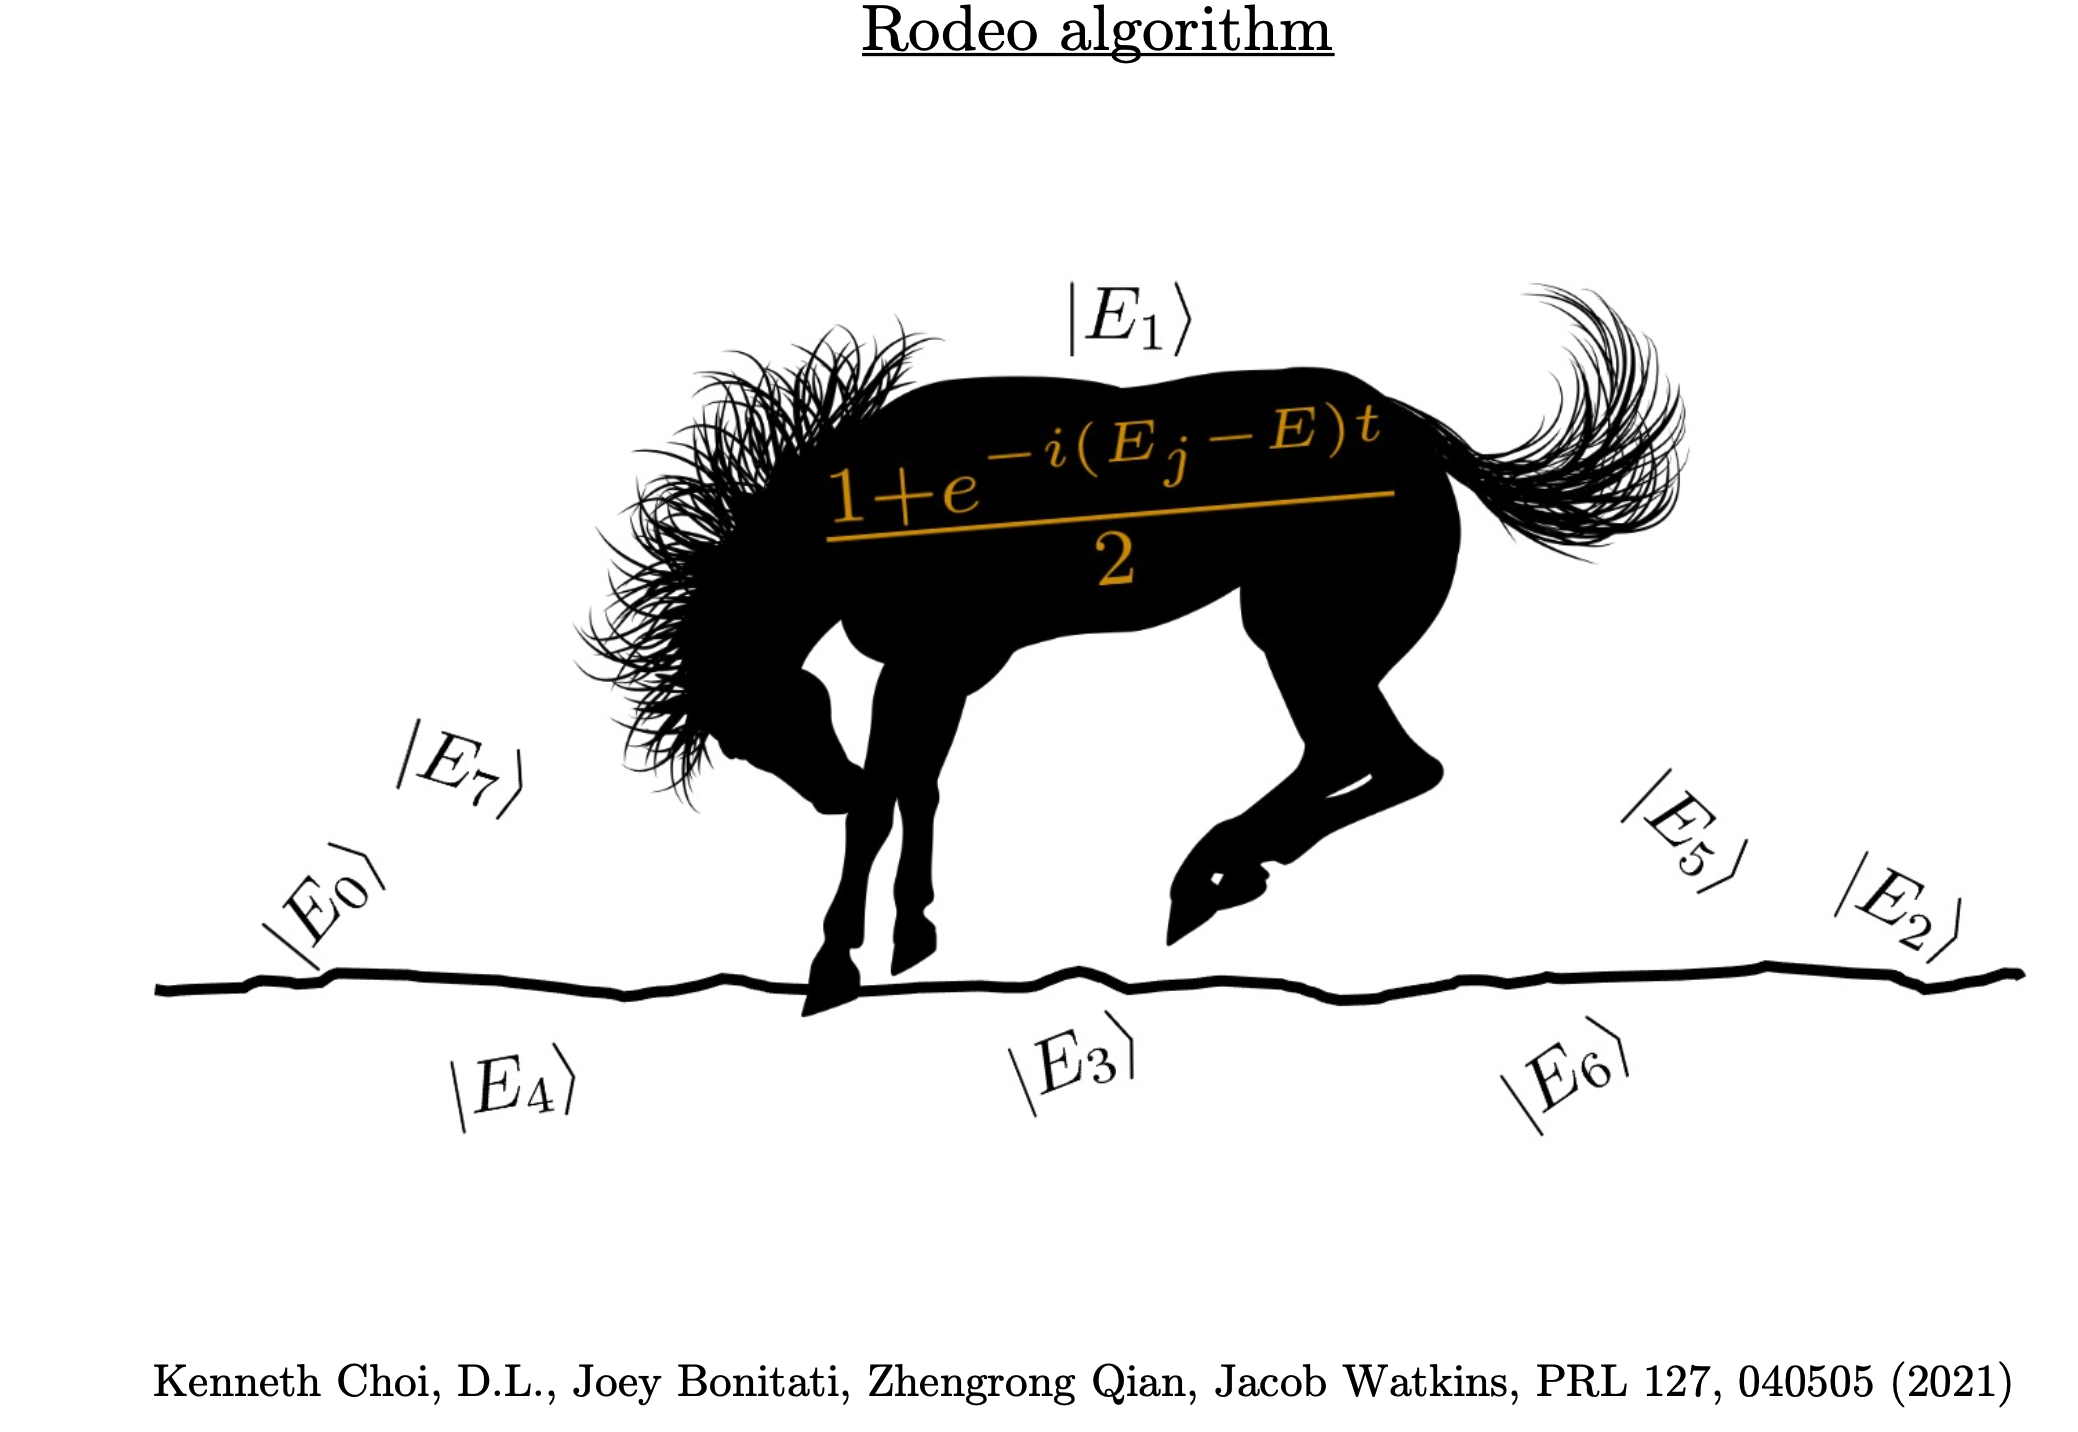
\includegraphics[width=1.05\linewidth]{rodeofigs/rodeo1.png}}
\end{frame}

\begin{frame}[plain,fragile]
\frametitle{What is this talk about?}

\begin{block}{Rodeo Algorithm}

In PRL {\bf 127} (2021), Choi {\em et al.,} presented a stochastic
quantum computing algorithm that can prepare any eigenvector of a
quantum Hamiltonian within a selected energy interval $[E-\epsilon, E+\epsilon]$.

In order to reduce the spectral
weight of all other eigenvectors by a suppression factor $\delta$, the
required computational effort scales as $O[|\log \delta|/(p\epsilon)]$, where $p$ is the squared overlap of the initial state
with the target eigenvector. The method uses auxiliary qubits to control the time evolution of the
Hamiltonian minus some tunable parameter $E$. With each auxiliary
qubit measurement, the amplitudes of the eigenvectors are multiplied
by a stochastic factor that depends on the proximity of their energy
to $E$. In this manner, one can converge to the target eigenvector with
exponential accuracy in the number of measurements.

\end{block}

\end{frame}

\begin{frame}[plain,fragile]
\frametitle{What is this talk about?}

\begin{block}{Rodeo Algorithm, more}

In addition to
preparing eigenvectors, the method can also compute the full spectrum
of the Hamiltonian.  For energy eigenvalue determination with error $\epsilon$,
the computational scaling is $O[(\log \epsilon)^2/(p \epsilon)]$.  For
eigenstate preparation, the computational scaling is $O(\log \Delta/p)$, where $\Delta$ is the magnitude of the orthogonal
component of the residual vector.  The speed for eigenstate
preparation is exponentially faster than that for phase estimation or
adiabatic evolution.
\end{block}

\end{frame}

\begin{frame}[plain,fragile]
\frametitle{The three steps of quantum control}
\begin{enumerate}
\item {\bf Quantum correlations:} Understanding and preparing an initial state
\item {\bf Quantum dynamics:} Controlled evolution towards a desired final state
\item {\bf Quantum measurements:} Measuring and characterizing the final state
\end{enumerate}
\end{frame}

\begin{frame}[plain,fragile]
\frametitle{Rodeo algorithm}

\begin{figure}
\centering
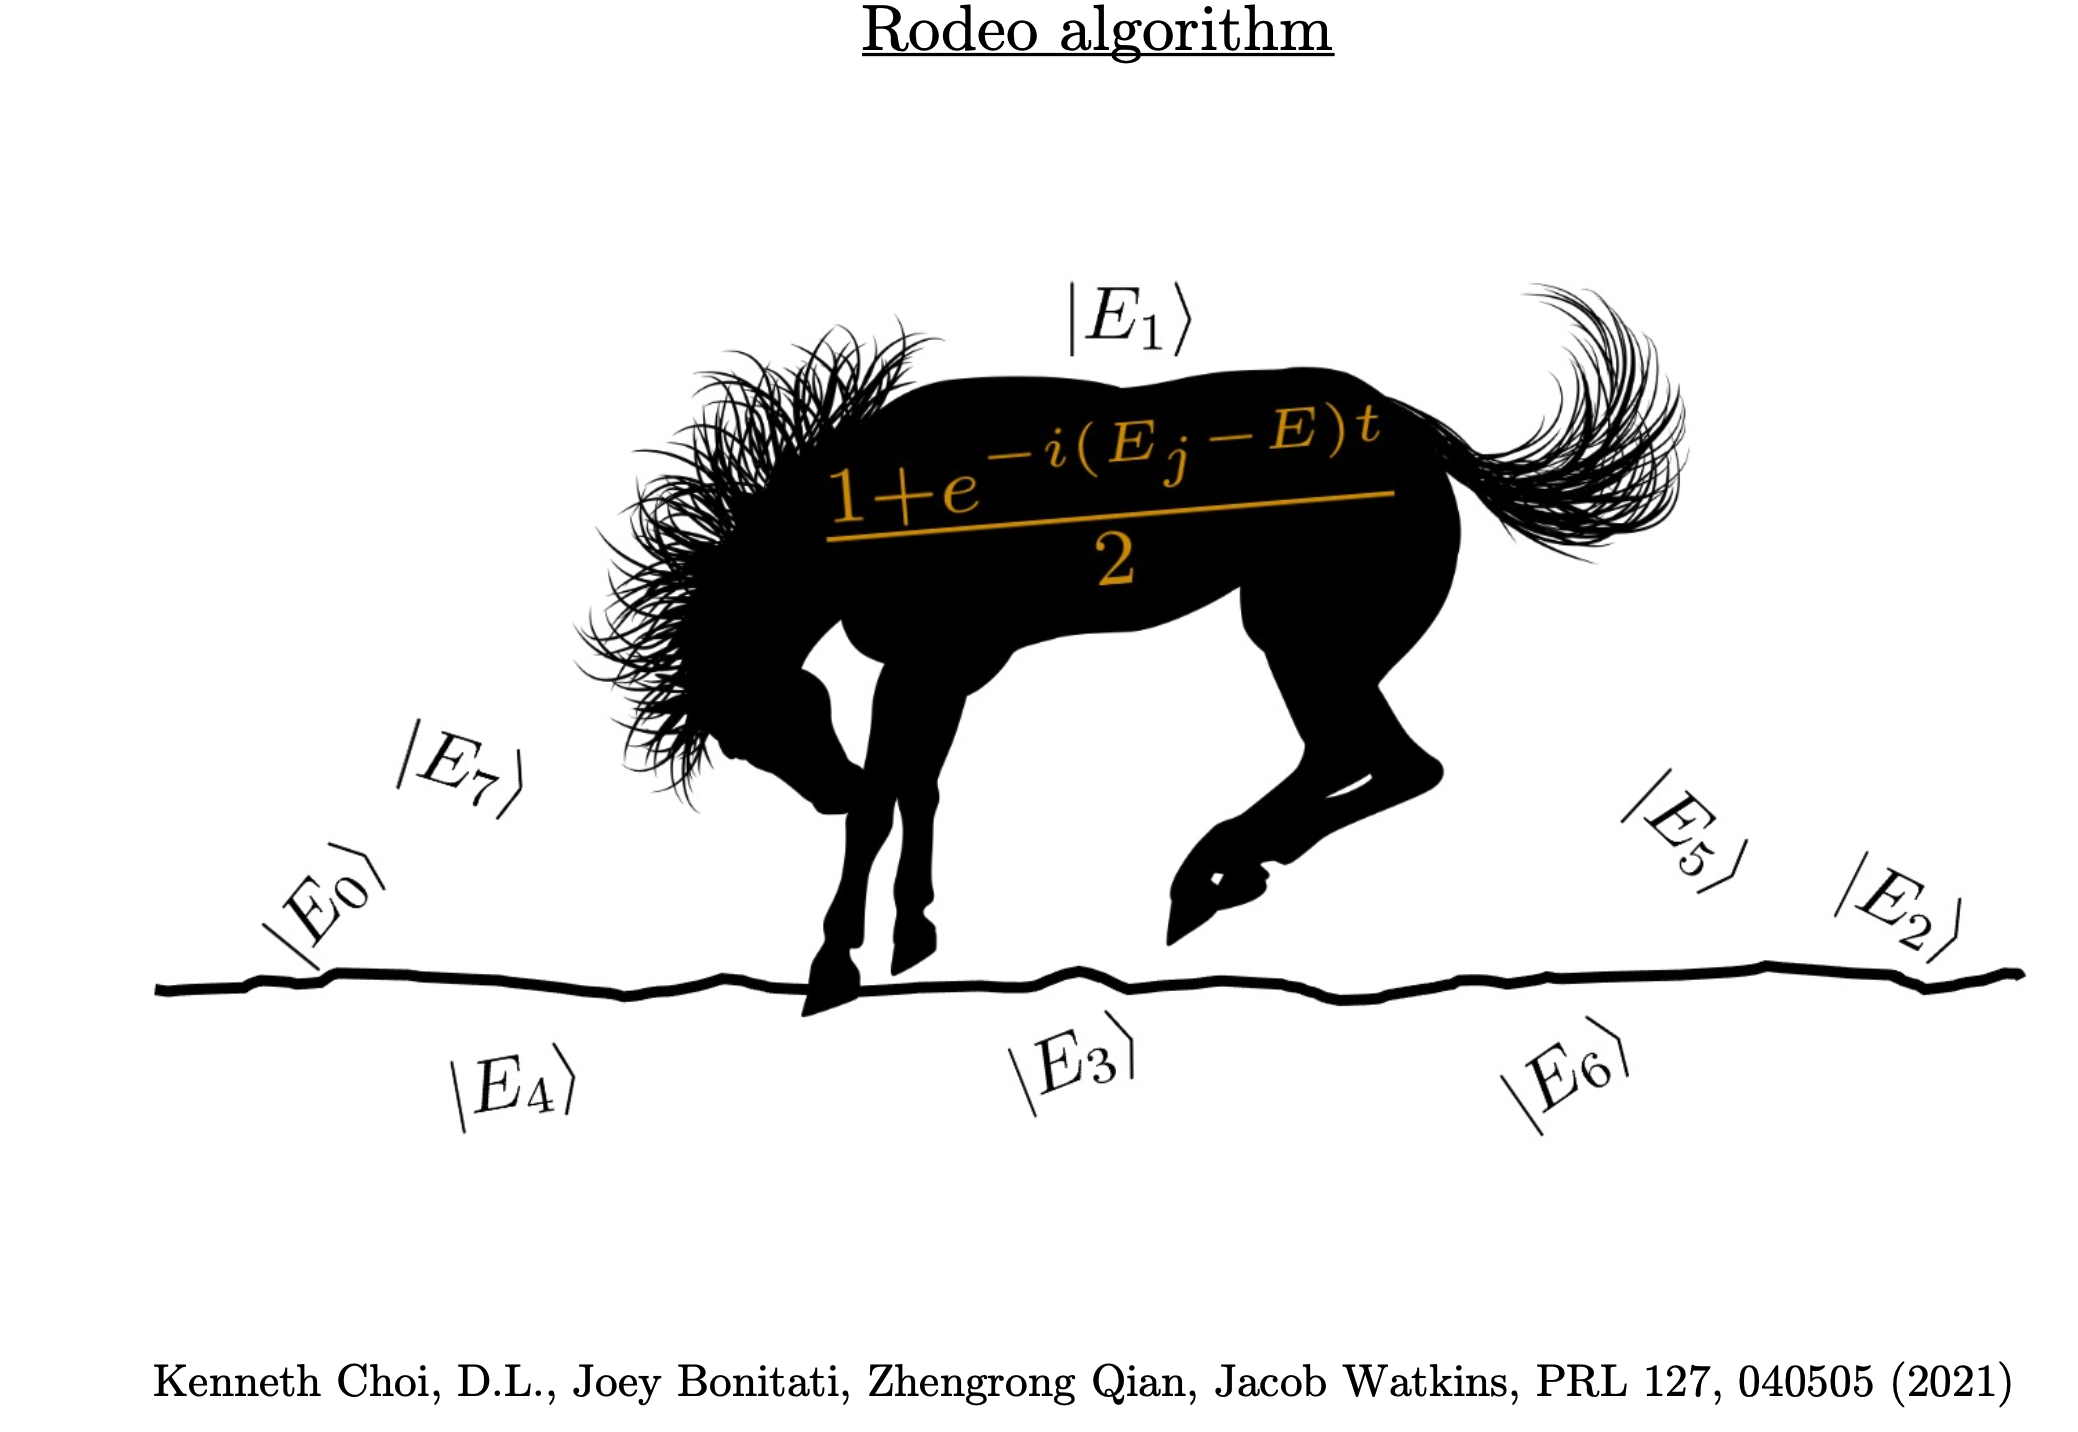
\includegraphics[width=9.5cm]{rodeofigs/rodeo1.png}
\end{figure} 

\end{frame}


\begin{frame}[plain,fragile]
\frametitle{Why is the Rodeo algorithm interesting?}
The rodeo algorithm operates by shaking off all other states until only the target eigenvector remains.
\begin{enumerate}
\item The rodeo algorithm has the advantage that it can be applied to any quantum Hamiltonian
\item It is a recursive algorithm that achieves exponential convergence in the number of cycles
\item It can be used to compute the full energy spectrum as well as prepare any energy eigenstate.
\end{enumerate}
\end{frame}

\begin{frame}[plain,fragile]
\frametitle{The Rodeo algorithm, as a figure}

\begin{figure}
\centering
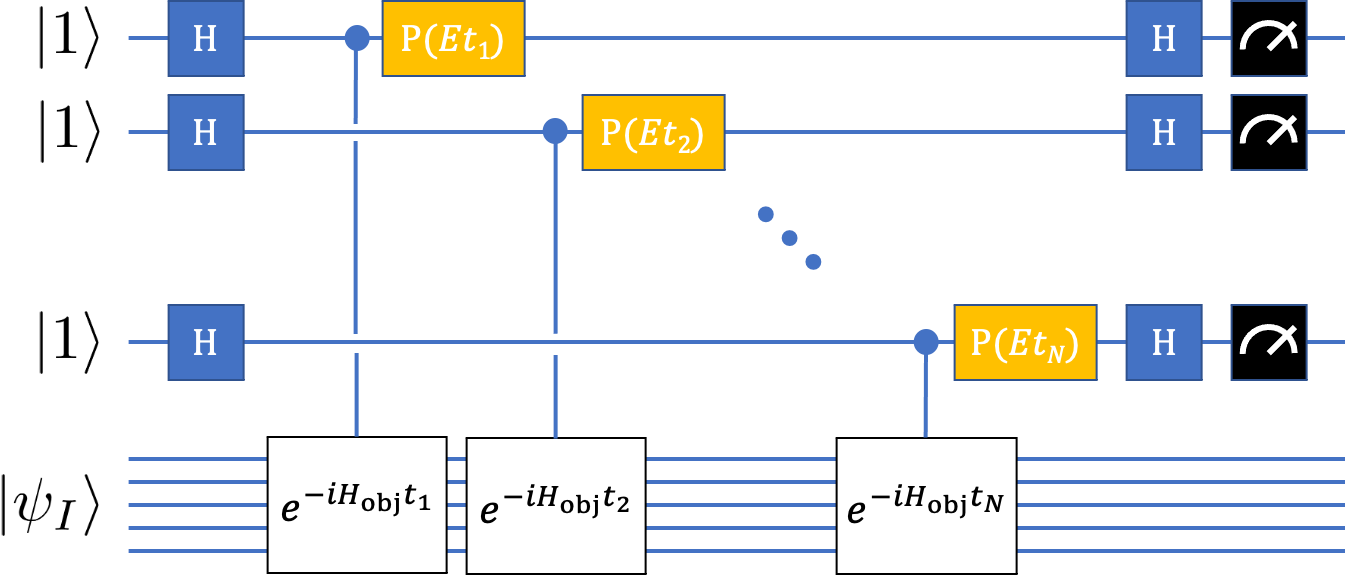
\includegraphics[width=8.5cm]{rodeofigs/rodeo_circuit.png}
\caption{(color online) {\bf Circuit diagram for the rodeo algorithm.} The object system starts in an arbitrary state $\ket{\psi_I}$.  Each of the ancilla qubits are initialized in the state $\ket{1}$ and operated on by a Hadamard gate H.  We use each ancilla qubit $n=1, \cdots, N$ for the controlled time evolution of the object Hamiltonian, $H_{\rm obj}$, for time $t_n$.  This is followed by a phase rotation P$(Et_n)$ on ancilla qubit $n$, another Hadamard gate H, and then measurement.}
\label{rodeo_circuit}
\end{figure} 

\end{frame}


\begin{frame}[plain,fragile]
\frametitle{The Rodeo algorithm, single qubit setup}
Consider first a Hadamard transformation on a single qubit
\[
H=\tfrac{1}{\sqrt{2}}\begin{bmatrix} 1 & 1 \\ 1 & -1\end{bmatrix},
\]
and a phase-rotation matrix
\[
P=\begin{bmatrix} 1 & 0 \\ 0 & e^{-\imath t(E_{\mathrm{obj}}-E)}\end{bmatrix}.
\]
We have then

\[
H^{\dagger}PH=\begin{bmatrix} \tfrac{1}{2}+\tfrac{1}{2}e^{-\imath t(E_{\mathrm{obj}}-E)} & \tfrac{1}{2}-\tfrac{1}{2}e^{-\imath t(E_{\mathrm{obj}}-E)} \\ \tfrac{1}{2}-\tfrac{1}{2}e^{-\imath t(E_{\mathrm{obj}}-E)}  & \tfrac{1}{2}+\tfrac{1}{2}e^{-\imath t(E_{\mathrm{obj}}-E)}\end{bmatrix}.
\]
\end{frame}



\begin{frame}[plain,fragile]
\frametitle{The Rodeo algorithm, single qubit start state}
Let us start in the state
\[
\begin{bmatrix} 0 \\ 1\end{bmatrix},
\]
and perform these unitary operations 
\[
H^{\dagger}PH\begin{bmatrix} 0 \\ 1\end{bmatrix} =\begin{bmatrix} \tfrac{1}{2}-\tfrac{1}{2}e^{-\imath t(E_{\mathrm{obj}}-E)} \\ \tfrac{1}{2}+\tfrac{1}{2}e^{-\imath t(E_{\mathrm{obj}}-E)}\end{bmatrix}.
\]
We project then back to the $\begin{bmatrix} 0 \\ 1\end{bmatrix}$ state 
\[
\begin{bmatrix} 0 & 0 \\ 0 & 1\end{bmatrix}H^{\dagger}PH\begin{bmatrix} 0 \\ 1\end{bmatrix} =\begin{bmatrix} 0\\ \tfrac{1}{2}+\tfrac{1}{2}e^{-\imath t(E_{\mathrm{obj}}-E)}\end{bmatrix}.
\]

\end{frame}

\begin{frame}[plain,fragile]
\frametitle{Projection of single qubit start state}

The above  projection is done via quantum measurement and the success
probability is
\[
\mathrm{Prob}(E_{\mathrm{obj}},E,t)= \left\vert\tfrac{1}{2}+\tfrac{1}{2}e^{-\imath t(E_{\mathrm{obj}}-E)}\right\vert^2=\cos^2{\left[\tfrac{t(E_{\mathrm{obj}}-E)}{2}\right]}
\]


\end{frame}


\begin{frame}[plain,fragile]
\frametitle{Convergence pattern}

\begin{figure}
\centering
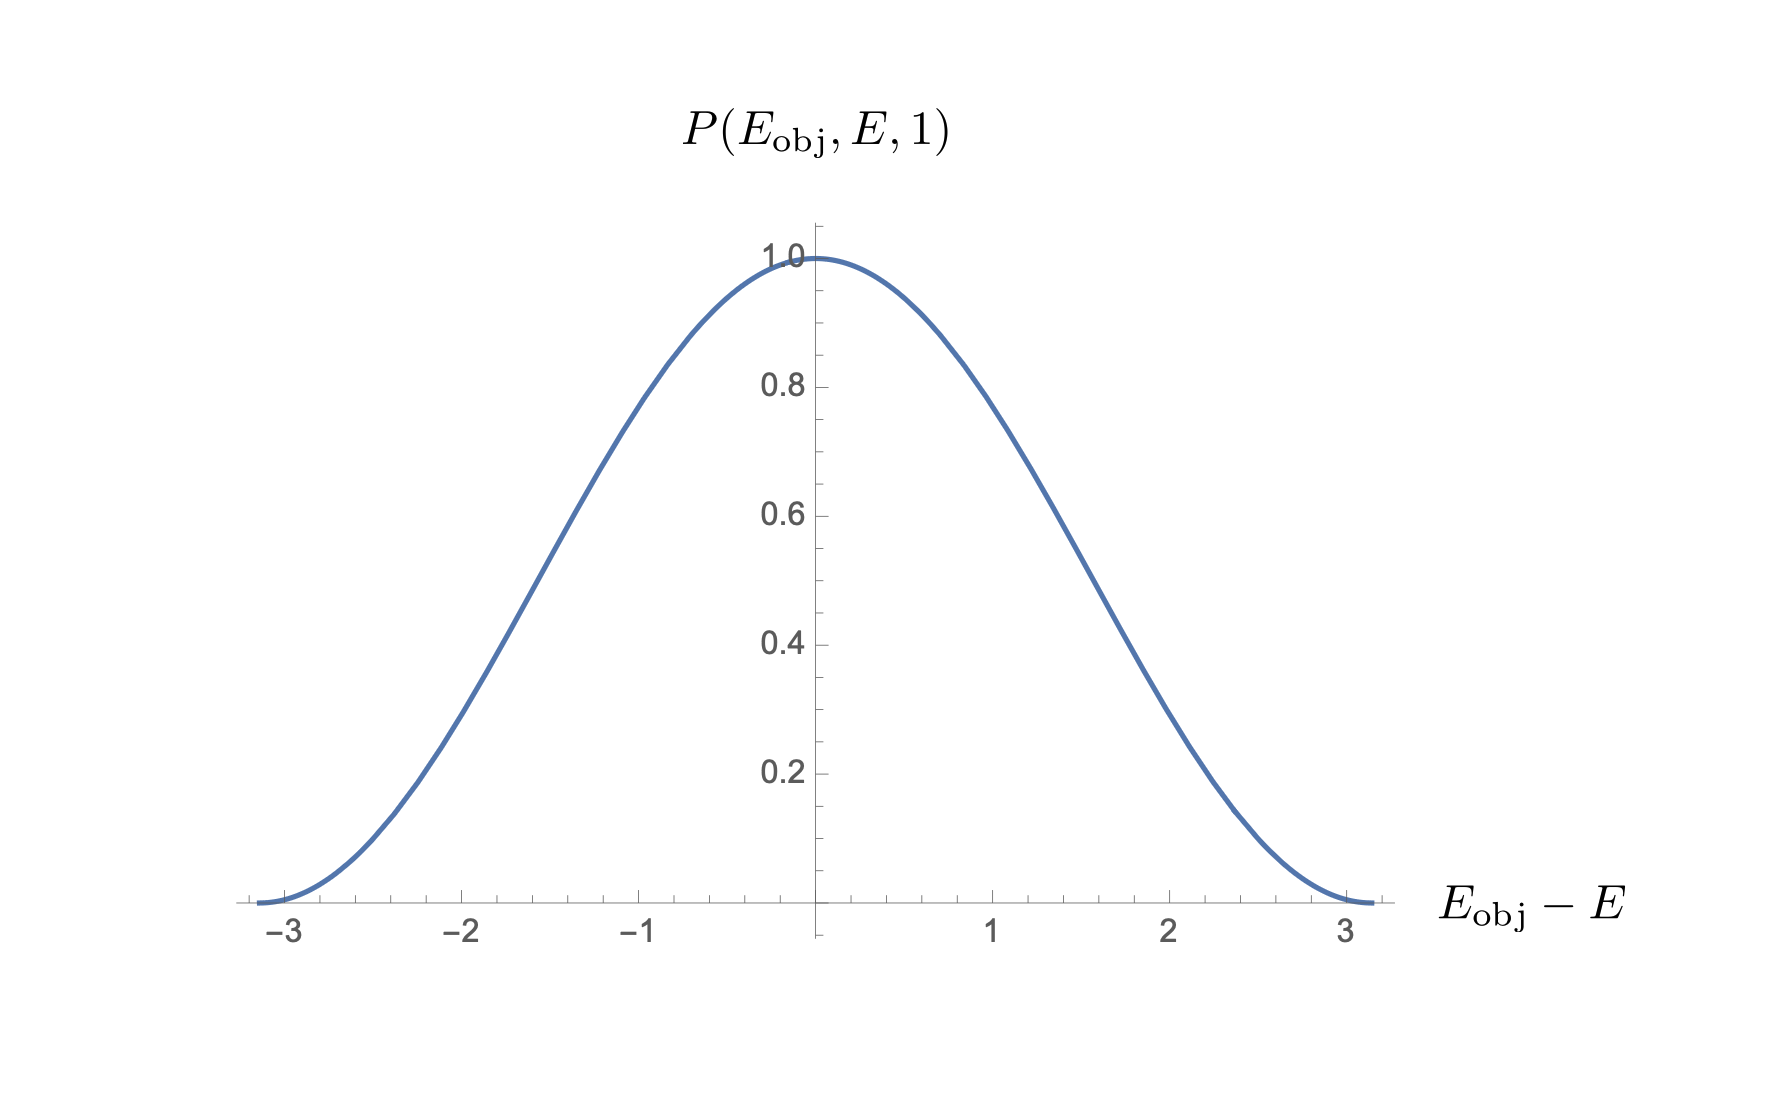
\includegraphics[width=8.5cm]{rodeofigs/rodeo2.png}
\end{figure} 

\end{frame}

\begin{frame}[plain,fragile]
\frametitle{Convergence pattern}

\begin{figure}
\centering
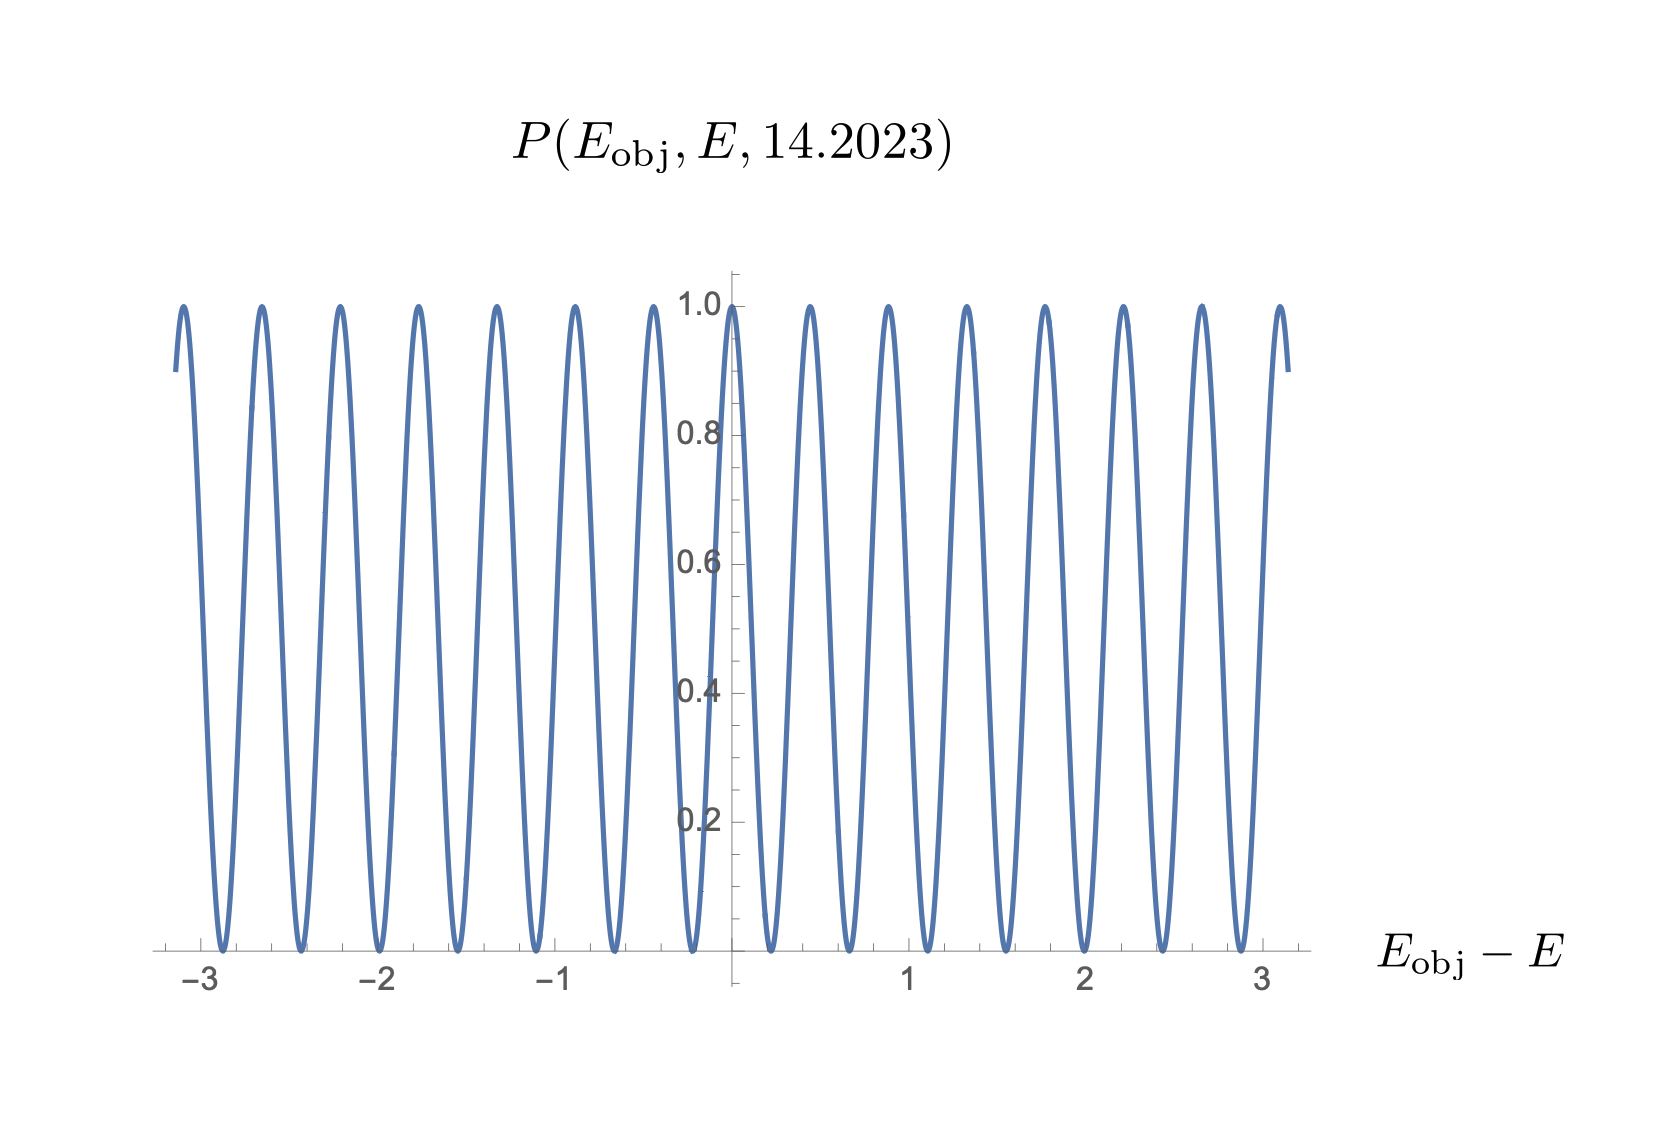
\includegraphics[width=8.5cm]{rodeofigs/rodeo3.png}
\end{figure} 

\end{frame}

\begin{frame}[plain,fragile]
\frametitle{Convergence pattern}

\begin{figure}
\centering
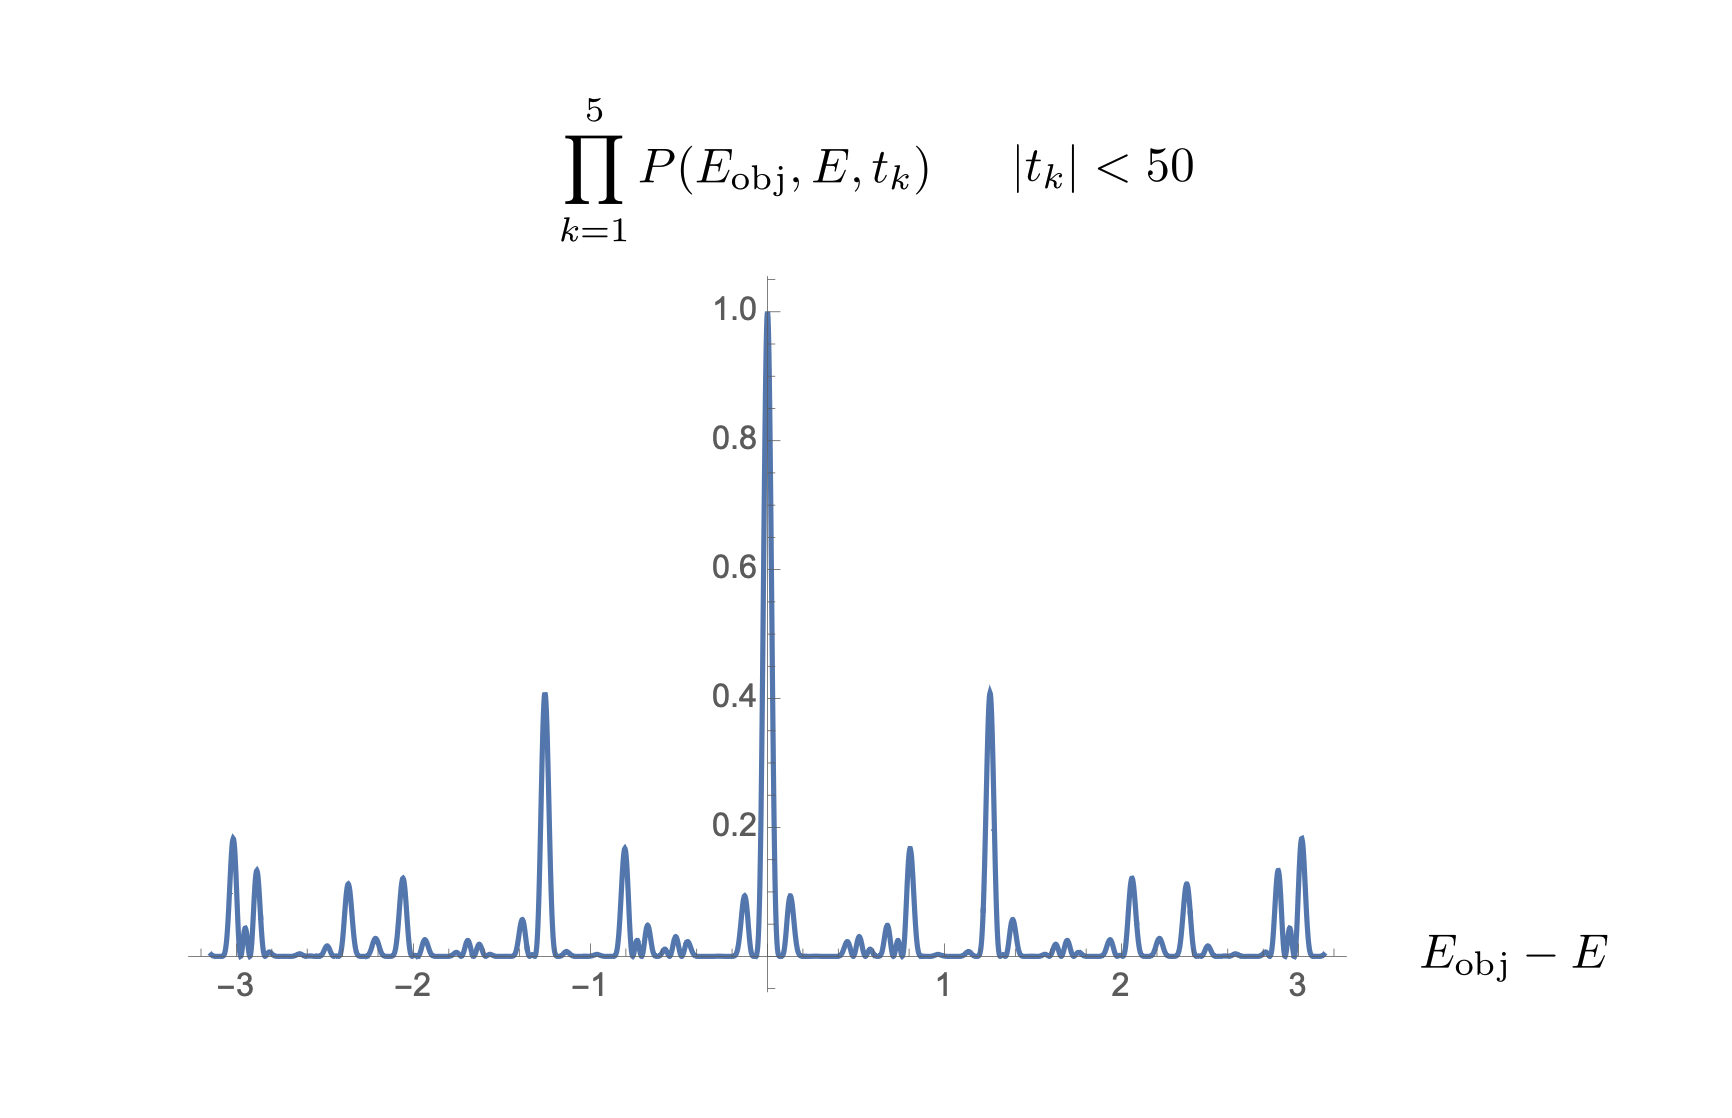
\includegraphics[width=8.5cm]{rodeofigs/rodeo4.png}
\end{figure} 

\end{frame}

\begin{frame}[plain,fragile]
\frametitle{Convergence pattern}

\begin{figure}
\centering
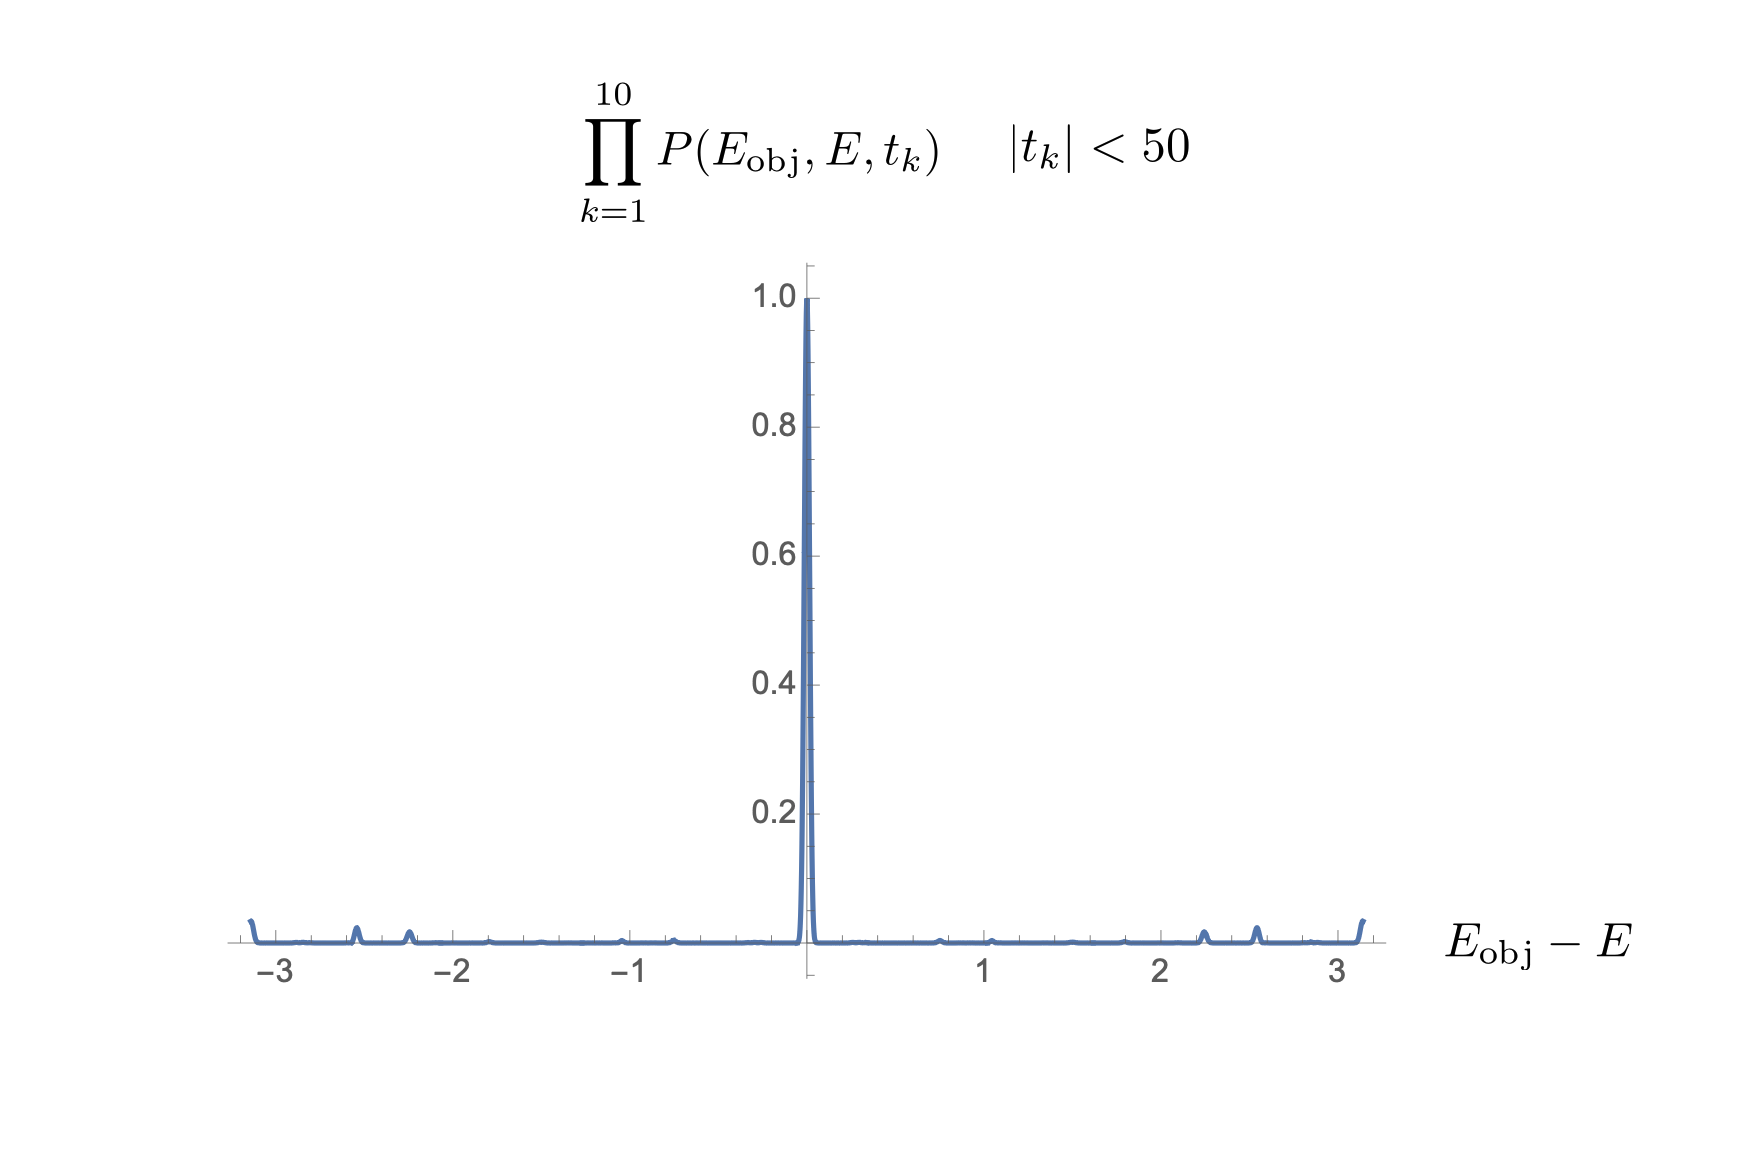
\includegraphics[width=8.5cm]{rodeofigs/rodeo5.png}
\end{figure} 

\end{frame}





\begin{frame}{Expanding to more qubits}
Let us couple this qubit, which we call the {\bf ancilla} qubit, to another
system that we call the {\bf object}. We also promote the $2\times 2$ matrices to
become $2\times 2$ matrices of operators acting on the object, that is 
\[
H=\tfrac{1}{\sqrt{2}}\begin{bmatrix} 1 & 1 \\ 1 & -1\end{bmatrix}\rightarrow\tfrac{1}{\sqrt{2}}\begin{bmatrix} \bm{I} & \bm{I} \\ \bm{I} & -\bm{I}\end{bmatrix},
\]
and the phase-rotation matrix
\[
P=\begin{bmatrix} 1 & 0 \\ 0 & e^{-\imath t(E_{\mathrm{obj}}-E)}\end{bmatrix}\rightarrow \begin{bmatrix} \bm{I} & 0 \\ 0 & e^{-\imath t(E_{\mathrm{obj}}-E)}\end{bmatrix}.
\]


\end{frame}

\begin{frame}{Expanding to more qubits, same transformations}

\[
H^{\dagger}PH=\tfrac{1}{\sqrt{2}}\begin{bmatrix} \bm{I} & \bm{I} \\ \bm{I} & -\bm{I}\end{bmatrix} \begin{bmatrix} \bm{I} & 0 \\ 0 & e^{-\imath t(E_{\mathrm{obj}}-E)}\end{bmatrix} \tfrac{1}{\sqrt{2}}\begin{bmatrix} \bm{I} & \bm{I} \\ \bm{I} & -\bm{I}\end{bmatrix},
\]


\end{frame}


\begin{frame}[plain,fragile]
\frametitle{The Rodeo algorithm, another start state}
Let us start in the state
\[
\begin{bmatrix} 0 \\ \ket{\psi_I}\end{bmatrix},
\]
and we perform the operations and then measure if the {\bf ancilla} qubit is in the $\begin{bmatrix} 0 \\ 1\end{bmatrix}$ state, that is  
we project then back to the $\begin{bmatrix} 0 \\ 1\end{bmatrix}$ state 
\[
\begin{bmatrix} 0 & 0 \\ 0 & \bm{I}\end{bmatrix}H^{\dagger}PH\begin{bmatrix} 0 \\ \ket{\psi_I}\end{bmatrix} =\begin{bmatrix} 0\\ \tfrac{1}{2}+\tfrac{1}{2}e^{-\imath t(E_{\mathrm{obj}}-E)}\ket{\psi_I}\end{bmatrix}.
\]

By repeated successful measurements with random values of $t$, we reduce
the spectral weight of eigenvectors with energies that do not match $E$.


\end{frame}



\begin{frame}[plain,fragile]
\frametitle{Probability of success}


The success probability of measuring all $N$ ancilla qubits in the $\ket{1}$ state is given by product, 
\[
   \mathrm{Prob}_N =\prod_{n=1}^N \cos^2\left[(E_{\rm obj}
   -E)\tfrac{t_n}{2}\right].
\]
Averaging over the Gaussian random times with $STD$ value $\sigma$ we get
\[
   \mathrm{Prob}_N =\left[\tfrac{1}{2}+\tfrac{1}{2}e^{-\imath t(E_{\mathrm{obj}}-E)}\right]^{N}.
\]

The convergence is exponential. For $N$ cycles of the rodeo algorithm, the
suppression factor for undesired energy states is $1/4N$

\end{frame}

\begin{frame}[plain,fragile]
\frametitle{The Rodeo algorithm, as a figure}

\begin{figure}
\centering
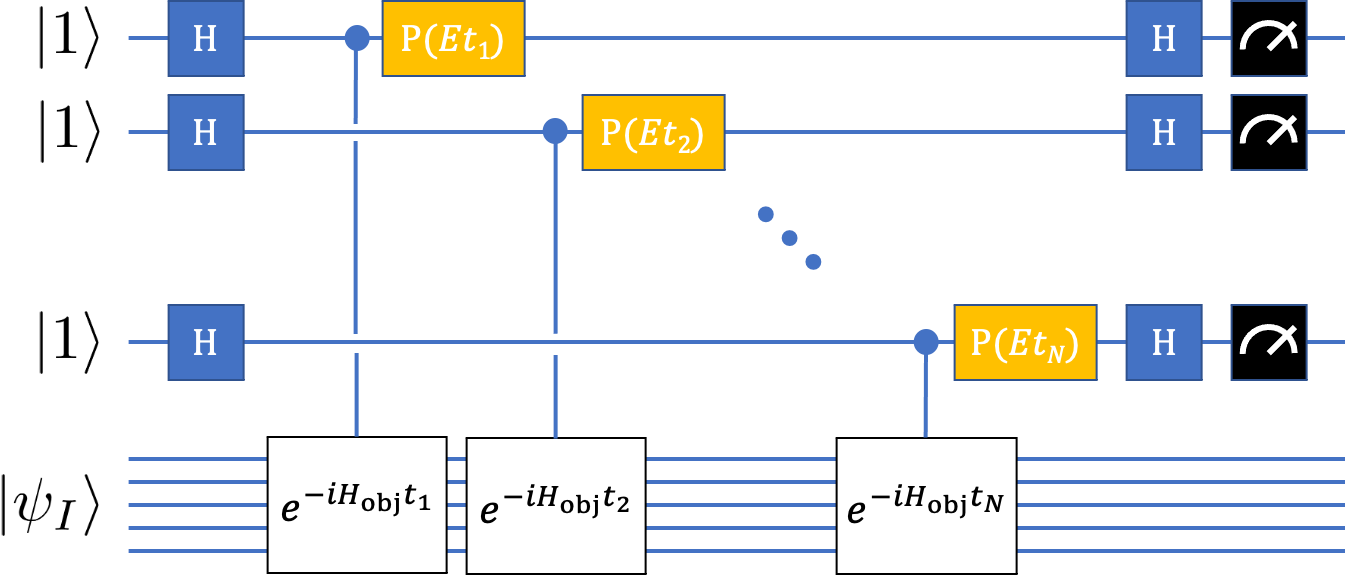
\includegraphics[width=8.5cm]{rodeofigs/rodeo_circuit.png}
\caption{(color online) {\bf Circuit diagram for the rodeo algorithm.} The object system starts in an arbitrary state $\ket{\psi_I}$.  Each of the ancilla qubits are initialized in the state $\ket{1}$ and operated on by a Hadamard gate H.  We use each ancilla qubit $n=1, \cdots, N$ for the controlled time evolution of the object Hamiltonian, $H_{\rm obj}$, for time $t_n$.  This is followed by a phase rotation P$(Et_n)$ on ancilla qubit $n$, another Hadamard gate H, and then measurement.}
\label{rodeo_circuit}
\end{figure} 

\end{frame}

\begin{frame}{More general expression}
\begin{itemize}
\item The Hamiltonian of interest is labelled as the object
Hamiltonian, $H_{\rm obj}$, and the linear space which it acts upon
the object system.

\item By assumption, the object system starts in some
initial state $\ket{\psi_I}$, which in general will update after each
measurement.

\item Use the auxiliary or ancilla qubits coupled to the object system.
\end{itemize}

\end{frame}

\begin{frame}{More general expression}

In order to illustrate the effect of these gate operations, let us
explicitly write out the operation for one cycle of the rodeo
algorithm with one ancilla qubit.  Starting from the initial state
$\ket{1} \otimes \ket{\psi_I}$ and performing one rodeo cycle, we
obtain


\begin{align*}
& \begin{bmatrix}
\left[ \tfrac{\bm{I}}{2}-\tfrac{1}{2}e^{-i(H_{\rm obj}-E)t_1} \right] \ket{\psi_I} \\
\left[ \tfrac{\bm{I}}{2}+\tfrac{1}{2}e^{-i(H_{\rm obj}-E)t_1} \right] \ket{\psi_I}
\end{bmatrix} =  \nonumber \\
& \begin{bmatrix}
\tfrac{\bm{I}}{\sqrt{2}} &
\tfrac{\bm{I}}{\sqrt{2}}\\
\tfrac{\bm{I}}{\sqrt{2}}& 
\tfrac{-I}{\sqrt{2}}
\end{bmatrix}
\begin{bmatrix}
 I & 0 \\
0 & Ie^{iEt_1} 
\end{bmatrix}
 \begin{bmatrix}
 I & 0 \\
0 & e^{-iH_{\rm obj}t_1}
\end{bmatrix} 
\begin{bmatrix}
\tfrac{\bm{I}}{\sqrt{2}} & 
\tfrac{\bm{I}}{\sqrt{2}}\\
\tfrac{\bm{I}}{\sqrt{2}} & 
\tfrac{-I}{\sqrt{2}}
\end{bmatrix}
\begin{bmatrix}
0 \\
\ket{\psi_I}
\end{bmatrix},
\label{one_rodeo}
\end{align*}
where $\bm{I}$ is the identity operator on the object system.


\end{frame}



\begin{frame}[plain,fragile]
\frametitle{Success probabilities}
We note that $H_{\rm obj}$ commutes with all of our gates, and so we can describe the action of the rodeo algorithm for each individual eigenvector of $H_{\rm obj}$ with energy $E_{\rm obj}$.  In that case, the probability of measuring the ancilla qubit $n$ in the $\ket{1}$ state is 
\[
   \cos^2\left[(E_{\rm obj}
   -E)\tfrac{t_n}{2}\right] = \left\vert \tfrac{1}{2}+
   \tfrac{1}{2}e^{-i(E_{\rm obj}-E)t_n} \right\vert^2.
\]
The success probability of measuring all $N$ ancilla qubits in the $\ket{1}$ state is given by the product 
\[
   \mathrm{Prob}_N =\prod_{n=1}^N \cos^2\left[(E_{\rm obj}
   -E)\tfrac{t_n}{2}\right]. 
\]
If we now take random values of $t_n$, we have an energy filter for $E_{\rm obj}=E$.  The geometric mean of $\cos^2\theta$ when sampled uniformly over all $\theta$ is equal to $\tfrac{1}{4}$.  Therefore the spectral weight for any $E_{\rm obj}\ne E$ is suppressed by a factor of $\tfrac{1}{4^N}$ for large $N$.


\end{frame}

\begin{frame}[plain,fragile]
\frametitle{Measurement probability}
\begin{figure}
\centering
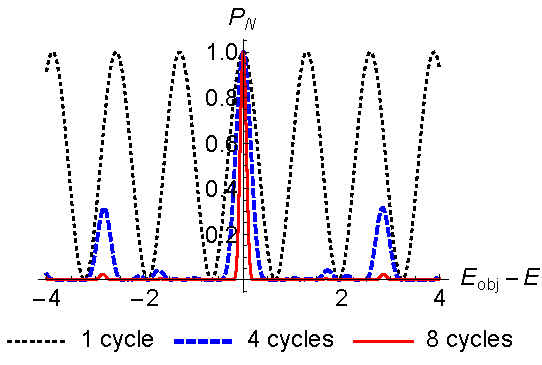
\includegraphics[width=8.0cm]{rodeofigs/rodeo_probability.pdf}
\caption{{\bf Measurement probability.} Probability $\mathrm{Prob}_N$ of measuring the $\ket{1}$ state for all ancilla qubits versus $E_{\rm obj}-E$ for $1$ (dotted black line), $4$ (dashed blue line), and $8$ (solid red line) cycles with Gaussian random values of $t_n$ with $t_{\rm RMS}=10$. If we use a Gaussian approximation for $\mathrm{Prob}_N$ near its maximum value of $1$ at $E_{\rm obj}=E$, we find that the width of the peak scales as $O[1/(\sqrt{N}t_{\rm RMS})]$.}
\label{rodeo_probability}
\end{figure} 

\end{frame}


\begin{frame}[plain,fragile]
\frametitle{Measurement probability}

Let $\epsilon$ be the desired energy resolution of our rodeo algorithm such that all energy eigenvectors outside of the interval $[E-\epsilon, E+\epsilon]$ are exponentially suppressed.
\begin{itemize}
\item If we choose $t_{\rm RMS}$ to scale proportionally with $1/\epsilon$, then we achieve the desired energy filtering with energy resolution $\epsilon$.
\item The actual peak width will be a factor of $1/\sqrt{N}$ narrower than $\epsilon$, but that is needed to get exponential suppression as a function of $N$ for all energies $E_{\rm obj}$ further than $\epsilon$ from $E$. 
\end{itemize}
\end{frame}



\begin{frame}[plain,fragile]
\frametitle{Measurement probability}
\begin{figure}
\centering
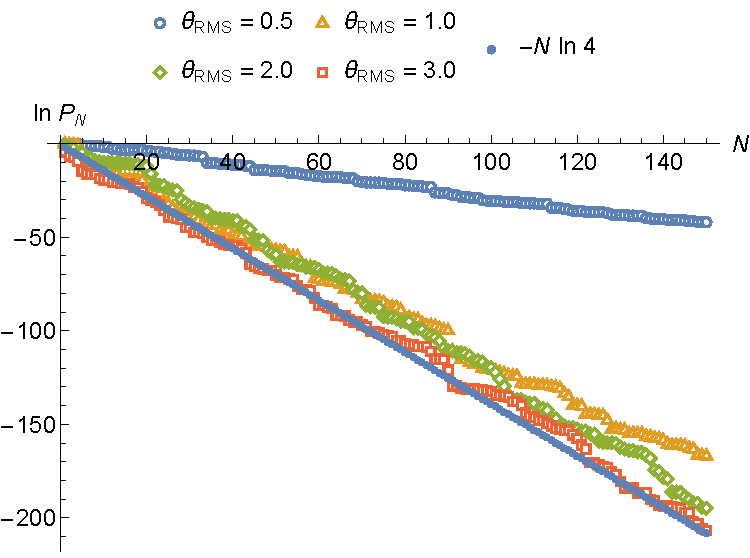
\includegraphics[width=8.0cm]{rodeofigs/Asymptotic.pdf}
\caption{{\bf Asymptotic scaling.} Plot of $\ln \mathrm{Prob}_N$ versus $N$ for Gaussian random values of $t_n$ with several selected values for $\theta_{\rm RMS}\equiv(E_{\rm obj}-E)\tfrac{t_{\rm RMS}}{2}$.  $\theta_{\rm RMS}=0.5$ (open circles), $\theta_{\rm RMS}=1.0$ (open triangles), $\theta_{\rm RMS}=2.0$ (open diamonds), and $\theta_{\rm RMS}=3.0$ (open squares). Predicted asymptotic scaling, $\ln \mathrm{Prob}_N = -N \ln 4$, with filled circles.}
\label{asymptotic}
\end{figure} 
\end{frame}

\begin{frame}[plain,fragile]
\frametitle{Measurement probability}
From the previous figure we  see that for $\theta_{\rm RMS}$ greater than $1$, the expected asymptotic scaling is achieved.  Therefore, if $t_{\rm RMS}$ is larger than twice the inverse spacing between energy levels, then $\mathrm{Prob}_N$ scales as $\tfrac{1}{4^N}$ for large $N$.
\end{frame}



\begin{frame}{Arbitrary initial state $\ket{\psi_I}$}
\begin{itemize}
\item Let $E_j$ be the energy eigenvalue nearest to $E$, and let $\ket{E_j}$ be the corresponding eigenvector. In the limit of large $N$, the probability that we measure the $\ket{1}$ state $N$ times in a row is $p\mathrm{Prob}_N$, where $p$ is the overlap probability of the initial state with $\ket{E_j}$, and $\mathrm{Prob}_N$ is the success probability for $E_{\rm obj}=E_j$. 

\item By tuning $E$ equal to $E_j$, this probability becomes $p$. If one requires that the spectral weights of all other energy eigenvectors outside the interval $[E-\epsilon,  E+\epsilon]$ are suppressed by a factor $\delta$, then the computational effort scaling for the rodeo algorithm is $N t_{\rm RMS}/p = O[|\log \delta|/(p \epsilon)]$. 

\end{itemize}

\end{frame}



\begin{frame}{Find any given energy eigenvalue $E_j$ with error $\epsilon$}
\begin{itemize}
\item The search process involves $O(\log \epsilon)$ sequential scans of the energy, each scan sweeping over an energy range that is some constant factor $K$ smaller than the previous scan.

\item Each scan is performed for several evenly spaced values of $E$, with a fixed number of rodeo cycles, and $t_{\rm RMS}$ a factor of $K$ larger than that used for the previous scan. 

\item The total time evolution required will scale as $O(1/\epsilon)$,  and the factor of $(\log \epsilon)^2/p$ comes from the required statistics needed to perform the energy scans successfully with high probability. The resulting performance as a function of $\epsilon$ is close to the $O(1/\epsilon)$ bound set by the Heisenberg uncertainty principle. 
\end{itemize}

\end{frame}



\begin{frame}{Prepare any given eigenstate $\ket{E_j}$ with a residual orthogonal component that has magnitude $\Delta$}
\begin{itemize}
\item Keep $t_{\rm RMS}$ fixed but large enough that we are filtering out only the desired eigenstate.

\item Perform $N = O(\log \Delta)$ cycles of the rodeo algorithm, must be multiplied by $1/p$ for the number of measurements required.

\item Keep $E$ centered on the peak maximum associated with $E_j$.  Re-centering $E$ with each cycle requires only a constant overall factor in the computational cost that is independent of $p$ and $\Delta$.
\end{itemize}

\end{frame}



\begin{frame}[plain,fragile]
\frametitle{Applications to the Heisenberg model}
As a first application of the rodeo algorithm, Choi et al., considered the spin-$\tfrac{1}{2}$ Heisenberg model in a uniform magnetic field with $10$ sites forming a
closed one-dimensional chain.  The Hamiltonian has the form
\begin{equation*}
    H_{\rm obj} = J \sum_{\braket{j,k}} \vec{\sigma}_j\cdot \vec{\sigma}_k + h \sum_{j} \sigma^z_j,
\end{equation*}
where $J$ is the exchange coupling, $\vec{\sigma}_j$ are the Pauli matrices on site $j$, $\braket{j,k}$ indicates nearest neighbors, and $h$ is the coupling to a uniform magnet\
ic field in the $z$ direction.  We consider the antiferromagnetic case with values $J=1$ and $h=3$. For our initial state we use an alternating tensor product state,
\begin{equation*}
    \ket{\psi_I} = \ket{0101010101}.
\end{equation*}
Since the initial state has a high degree of symmetry, one can expect that the initial state to have nonzero overlap with a relatively small number of energy eigenstates.

\end{frame}

\begin{frame}[plain,fragile]
\frametitle{Heisenberg model}
\begin{figure}
\centering
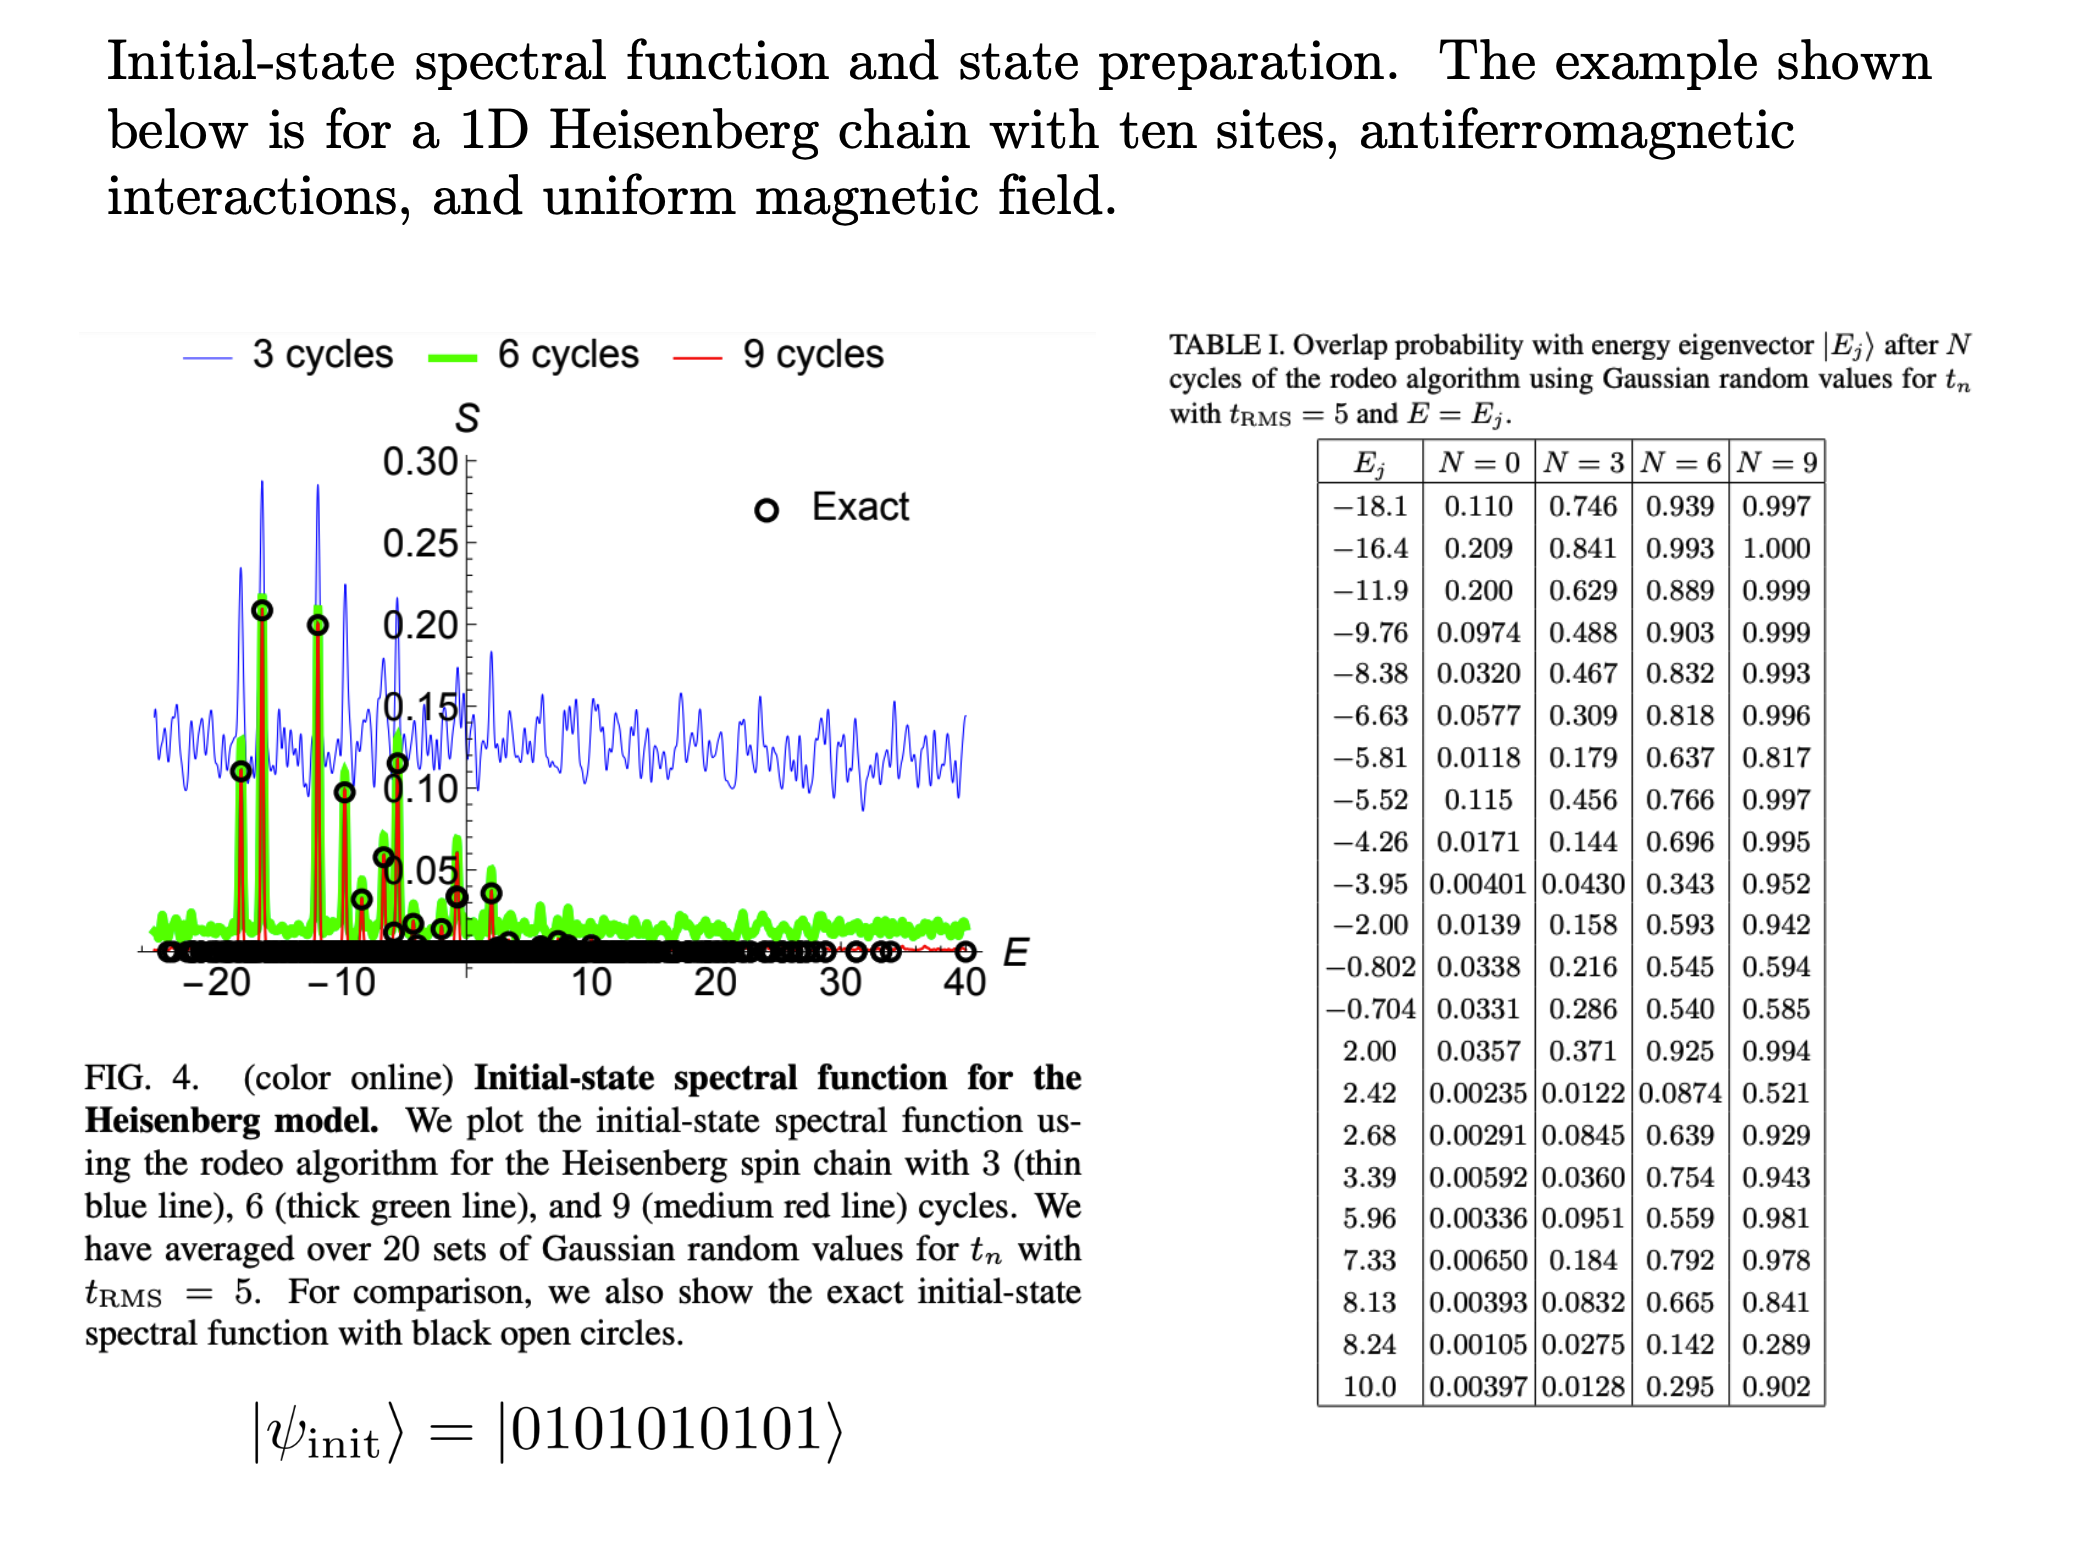
\includegraphics[width=10.0cm]{rodeofigs/rodeo6.png}
%\caption{{\bf Initial-state spectral function for the Heisenberg model.} We plot the initial-state spectral function using the rodeo algorithm for the Heisenberg spin chain with $3$ (thin blue line), $6$ (thick green line), and $9$ (medium red line) cycles. We have averaged over $20$ sets of Gaussian random values for $t_n$ with $t_{\rm RMS}=5$.  For comparison, we also show the exact initial-state spectral function with black open circles.}
\label{Heisenberg_spectrum}
\end{figure} 

\end{frame}


\begin{frame}[plain,fragile]
\frametitle{Log of wave function error}
\begin{figure}
\centering
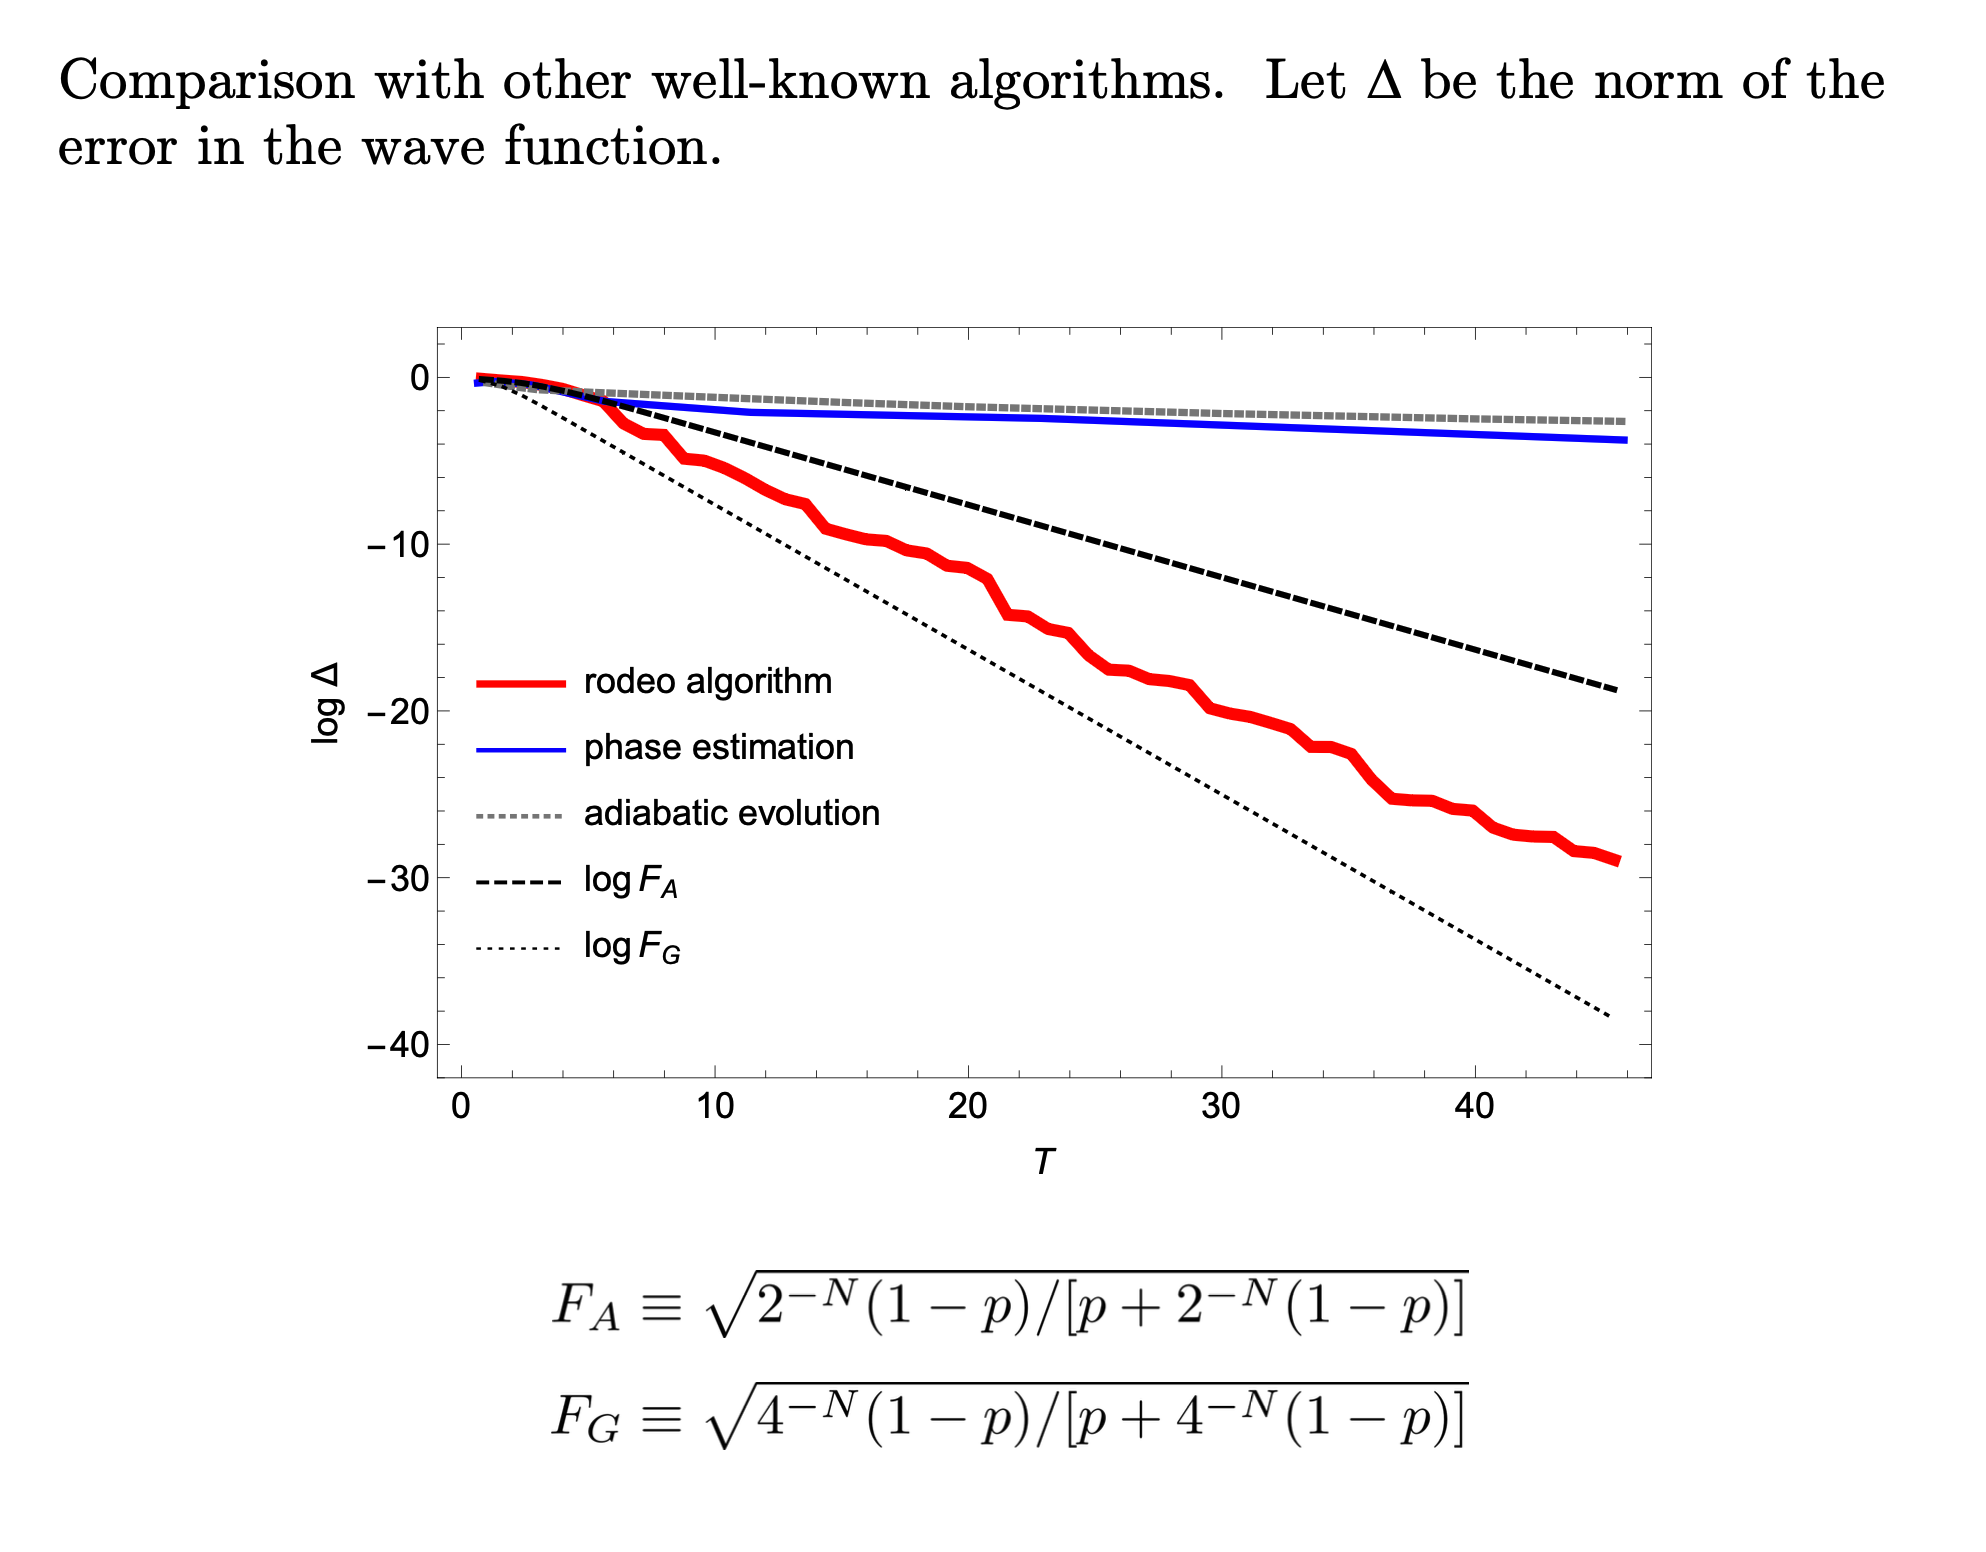
\includegraphics[width=10.5cm]{rodeofigs/rodeo7.png}
%\caption{{\bf Initial-state spectral function for the Heisenberg model.} We plot the initial-state spectral function using the rodeo algorithm for the Heisenberg spin chain with $3$ (thin blue line), $6$ (thick green line), and $9$ (medium red line) cycles. We have averaged over $20$ sets of Gaussian random values for $t_n$ with $t_{\rm RMS}=5$.  For comparison, we also show the exact initial-state spectral function with black open circles.}
\label{Heisenberg_spectrum}
\end{figure} 

\end{frame}


\begin{frame}[plain,fragile]
\frametitle{Implementation on real quantum computer}
\begin{figure}
\centering
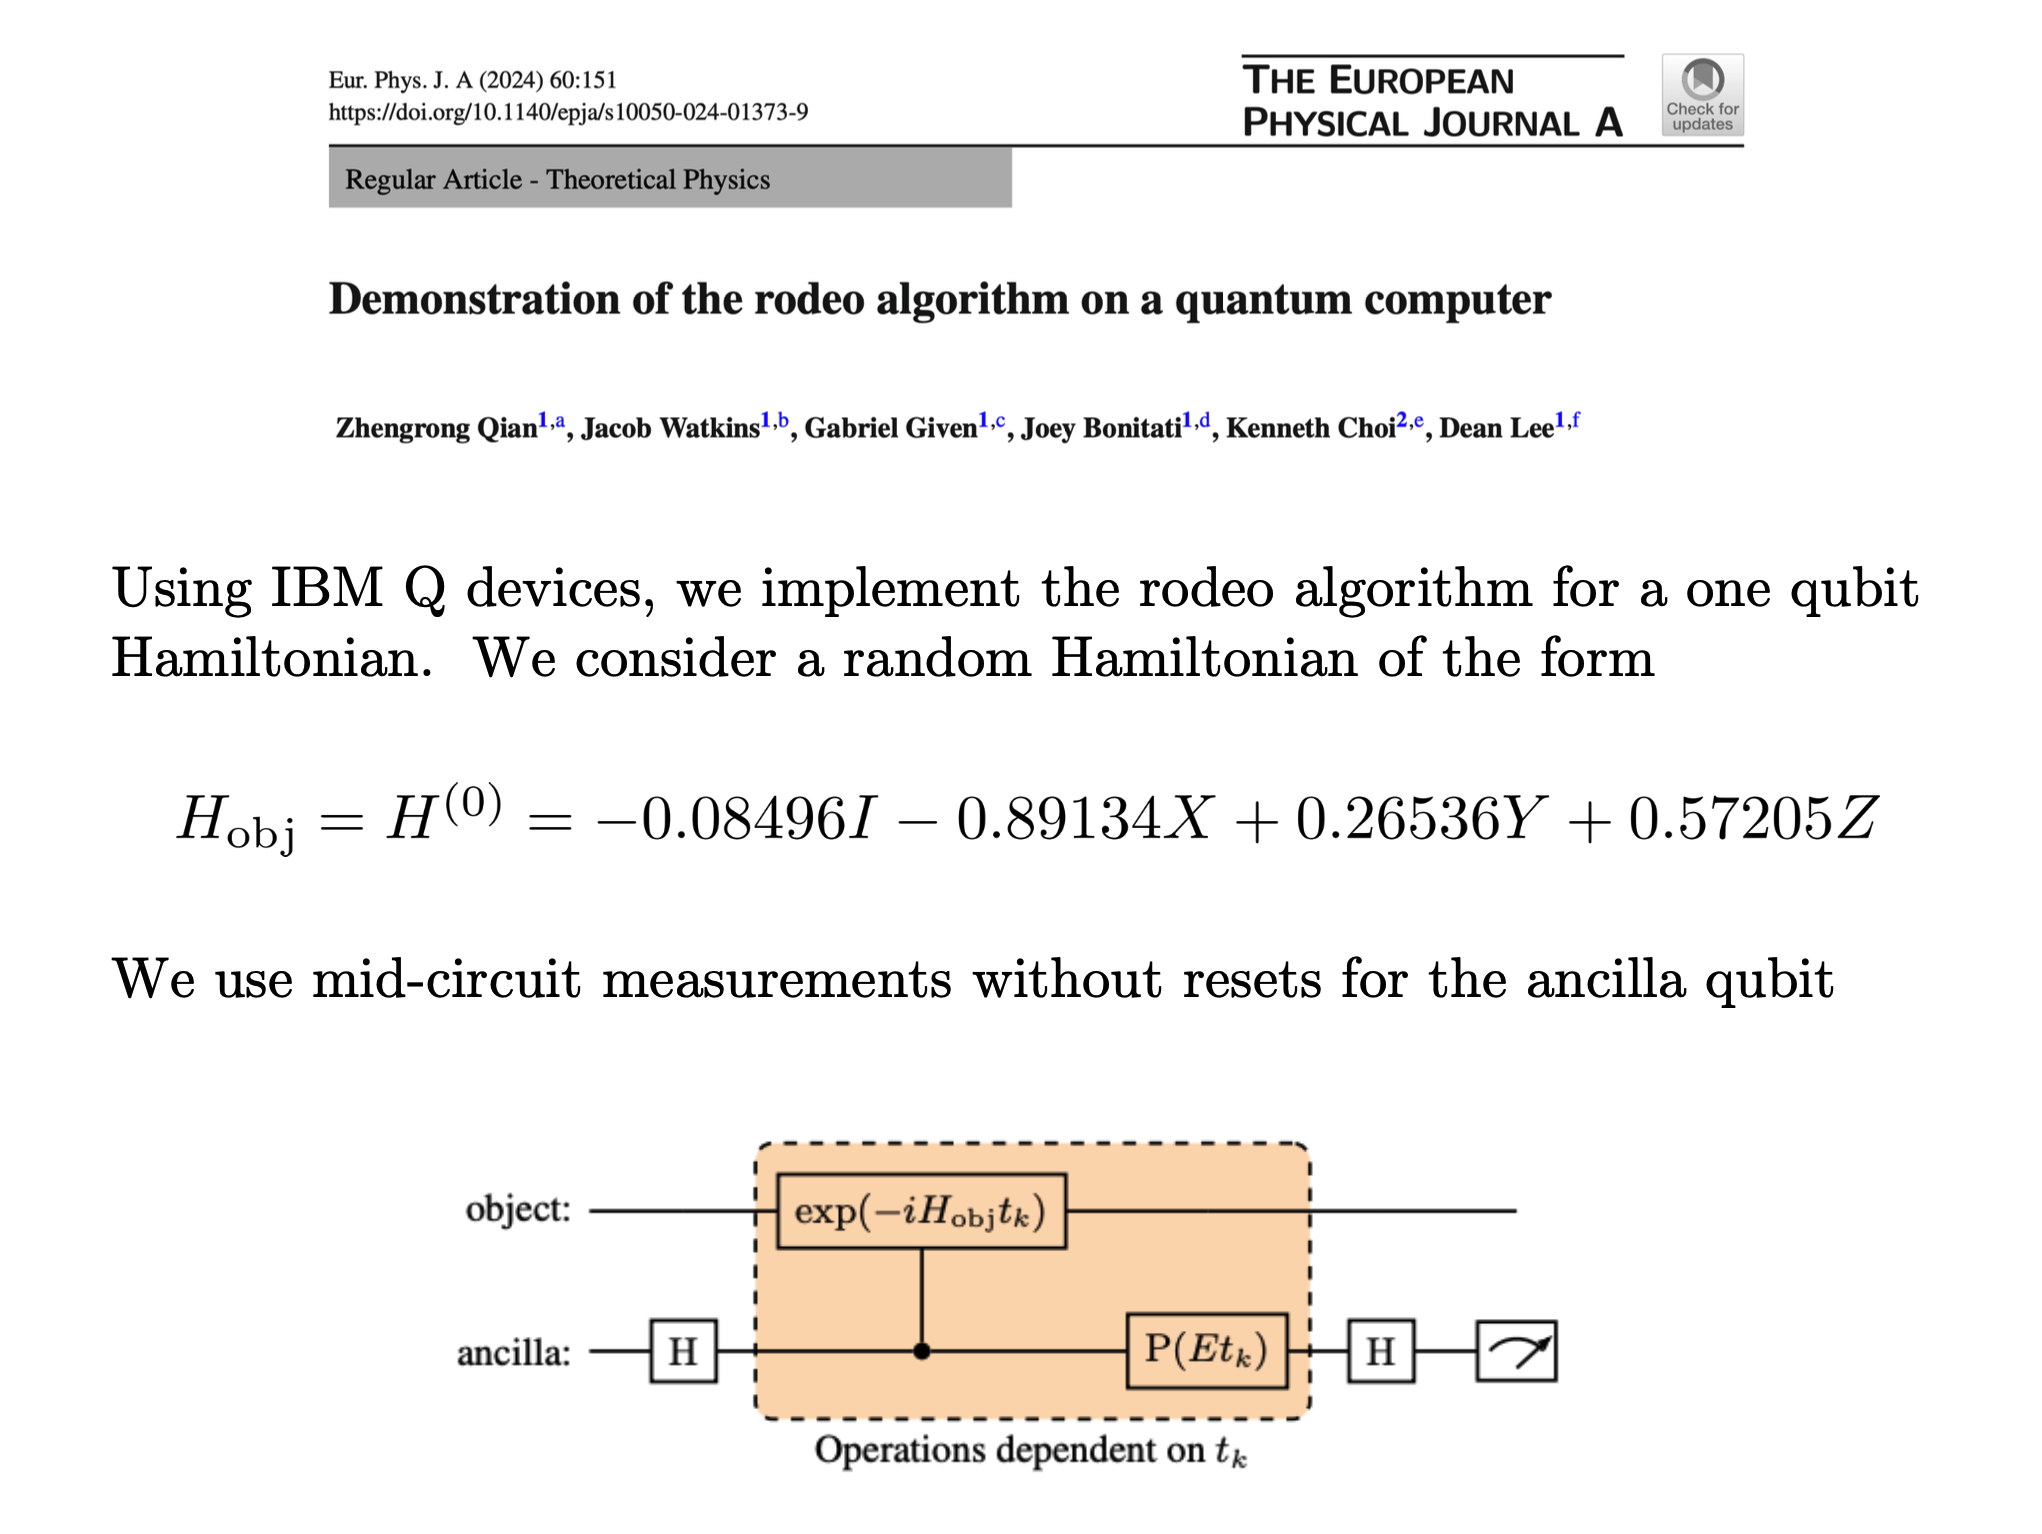
\includegraphics[width=8.5cm]{rodeofigs/rodeo9.png}
%\caption{{\bf Initial-state spectral function for the Heisenberg model.} We plot the initial-state spectral function using the rodeo algorithm for the Heisenberg spin chain with $3$ (thin blue line), $6$ (thick green line), and $9$ (medium red line) cycles. We have averaged over $20$ sets of Gaussian random values for $t_n$ with $t_{\rm RMS}=5$.  For comparison, we also show the exact initial-state spectral function with black open circles.}
\label{Heisenberg_spectrum}
\end{figure} 

\end{frame}



\end{document}







 









